\chapter{Marco teórico}
\TODO{Un overview del marco teórico}
\section{Estructura estelar Newtoniana}
\REMARK{Una de las razones para incluir el caso Newtoniano es que permite interpretar luego las ecuaciones obtenidas en relatividad general.}
Se presentarán las ecuaciones de estructura estelar Newtonianas puesto que esto facilita la interpretación de las ecuaciones de estructura que se obtendrán en relatividad general.

Considerando/partiendo una distribución de materia con simetría esférica, si $r$ denota la distancia desde el centro de la configuración, la masa $m(r)$ encerrada en una esfera/superficie esférica de radio $r$ será:  
\begin{equation}
    m ( r ) = \int _ { 0 } ^ { r } 4 \pi r ^ { 2 } \rho \mathrm{d} r = \int_{0}^{r} \mathrm{d}m(r) \quad\text{con}\quad \dd{m(r)}=4\pi r^2\rho,
\end{equation}
de donde
\begin{equation}
    \dv{m(r)}{r} =4\pi r^2 \rho.
    \label{dmnewton}
\end{equation}
Ahora, se considera un cilindro infinitesimal a una distancia $r$ del centro, de altura $\mathrm{d}r$ y sección transversal unitaria, normal al vector posición $\vec{r}$ (ver Figura \ref{stellnew}).   

\begin{figure}[H]
    \centering
    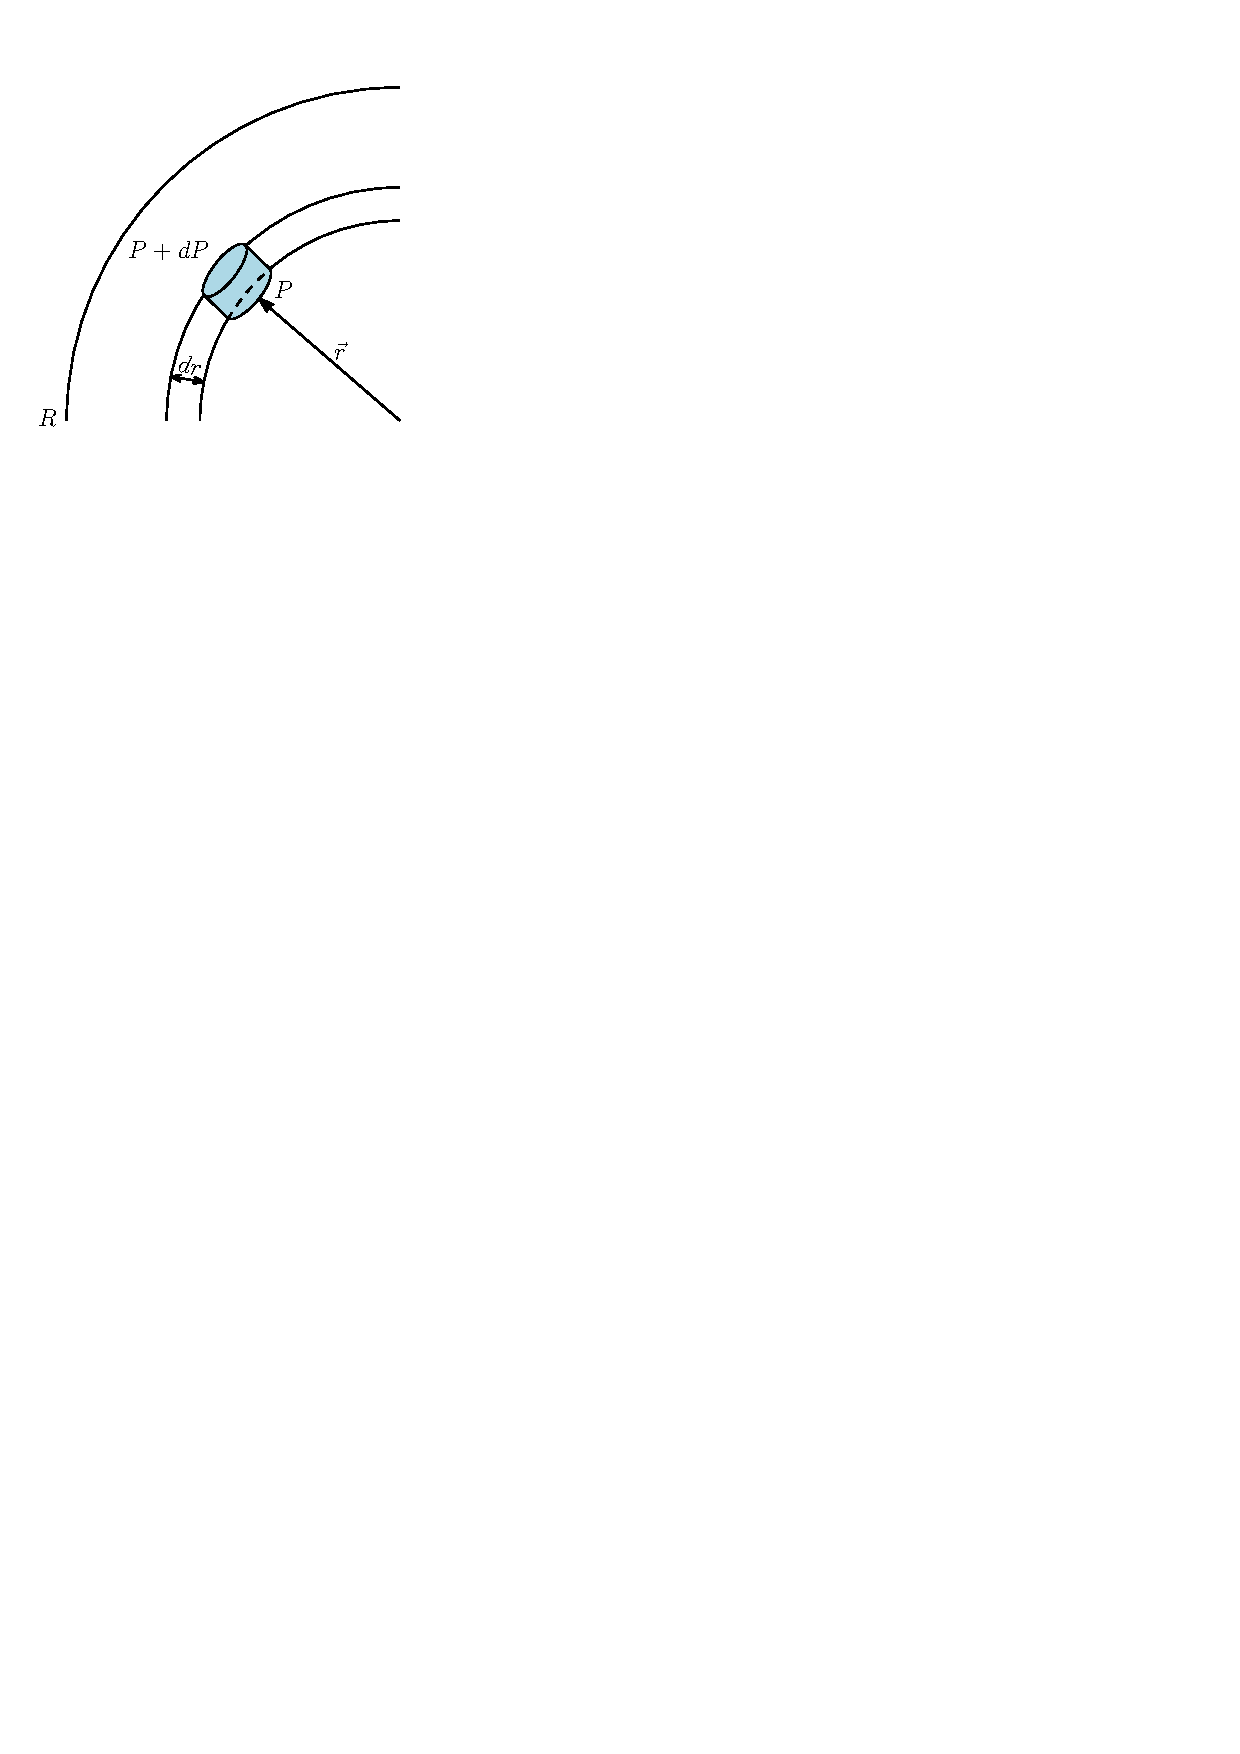
\includegraphics[width=150pt]{figures/stellarnewton.pdf}
    \caption{Presión sobre un elemento de masa cilíndrico.}
    \label{stellnew}
\end{figure}
Si la presión en $\vec{r}$ es $P$ y su cambio al ir de $\vec{r}$ a $\vec{r}+\mathrm{d}\vec{r}$ es $\mathrm{d}P$, esta diferencia de presión representa una fuerza $-\dd P$ (dado que la sección transversal es unitaria) actuando sobre el elemento de masa. Esta fuerza debe ser contrarrestada por la atracción gravitacional sobre el elemento de masa debido a $m(r)$ ($G m(r) \rho \dd r/r^2$) para que éste se encuentre en equilibrio:

\begin{equation}
    -\dd P =\frac{Gm(r)\rho\dd r}{r^2},
\end{equation}
o equivalentemente
\begin{equation}
    \frac { d P } { d r } = - \frac { G m ( r ) } { r ^ { 2 } } \rho.
    \label{dpnewton}
\end{equation}

Las ecuaciones \eqref{dmnewton} y \eqref{dpnewton} son las ecuaciones de estructura estelar Newtonianas \cite{Chandrasekhar1958AnStructure}, si una relación entre la presión y la densidad $P(\rho)$ es dada, es decir, una ecuación de estado, el sistema puede resolverse dado un par condiciones iniciales $m(r=0)$ y $P(r=0)$. La primera de estas condiciones es evidente puesto que no hay masa encerrada en un cascarón esférico de radio nulo, $m(r=0)=0$ y la segunda estará definida por el valor de $\rho(r=0)\equiv\rho_c$ escogido, mediante la ecuación de estado, $P(r=0)=P(\rho_c)$.

El radio de la estrella $R$ se define como el valor de $r$ en el que la presión se anula, esto es, $P(R)=0$ y de manera similar la masa de la estrella $M$ se define como el valor de la masa encerrada en $r=R$, esto es, $m(R)=M$.

Aunque no se van a tratar en el trabajo de grado, cabe resaltar que los objetos compactos conocidos como enanas blancas, sostenidas al igual que las estrellas de neutrones por la presión de degeneración no de neutrones sino de electrones, son bien descritas por las ecuaciones de estructura Newtonianas. Una manera, aunque no la única, de conocer la importancia de las correcciones relativistas es comparando la magnitud del potencial gravitacional con la unidad, con masas en un rango de $0.33\,M_{\odot}$ $1.52\,M_{\odot}$ y radios típicos de unos cuantos miles de kilómetros \cite{Glendenning2000CompactStars}, para las enanas blancas se cumple
\begin{equation}
    \frac{2GM}{c^2R}\ll 1,
\end{equation}
por lo cual se espera que el tratamiento Newtoniano sea suficiente \cite{Weinberg1972GravitationCosmology}. \TODO{Pulir último párrafo, parece redundante.}

\section{Estructura estelar relativista}

Si bien en la teoría Newtoniana podrían existir objetos tan compactos como las estrellas de neutrones, Chandrasekhar encontró que las estrellas soportadas por presión de degeneración tienen una masa máxima, obtenida asintóticamente cuando los Fermiones son altamente relativistas, esto es, cuando tienen velocidades comparables con la velocidad de la luz. Bajo tales condiciones existirían estrellas compuestas por los quarks más pesados (charm, bottom y top), que no son realizables en relatividad general debido a que las estrellas con la máxima masa posible no son lo suficientemente densas \cite{Glendenning2000CompactStars}.

Es por predicciones erróneas como la anterior que la relatividad general es necesaria para el estudio de objetos compactos, siendo precisamente el descubrimiento de los pulsares, estrellas de neutrones altamente magnetizadas en rotación, en 1967 \cite{Hewish1968ObservationSource} lo que revitalizó el estudio de la relatividad general y la llevó a la frontera de la investigación en física.\REMARK{Esto se podría trasladar a la introducción.}

Para describir la estructura de una estrella estática en relatividad general se supone un espacio-tiempo estático e isótropo descrito de manera general por la métrica asociada al elemento de línea:

\begin{equation}
\mathrm { d } s ^ { 2 } = e ^ { 2 \nu ( r ) } \mathrm { d } t ^ { 2 } - e ^ { 2 \lambda ( r ) } \mathrm { d } r ^ { 2 } - r ^ { 2 } \left( \mathrm { d } \theta ^ { 2 } + \sin ^ { 2 }  \theta  \mathrm { d } \phi ^ { 2 } \right) .   
\end{equation}

Además el espacio-tiempo se dividirá en dos: una región exterior a la estrella y una región interior. 
La \textit{región exterior} es libre de fuentes ($T _ { \mu } ^ { \nu }=0$) y las ecuaciones de Einstein para esta, en unidades gravitacionales ($G=c=1$), son 

\begin{equation}
    G _ { \mu } ^ { \nu } = R _ { \mu } ^ { \nu } - \frac { 1 } { 2 } g _ { \mu } ^ { \nu } R = 8 \pi T _ { \mu } ^ { \nu }=0,
\end{equation}
de donde se obtiene
\begin{equation}
    e ^ { 2 \nu } = 1 - \frac { 2 M } { r };\quad \quad - e ^ { 2 \lambda } = - e ^ { - 2 \nu } = - \left( 1 - \frac { 2 M } { r } \right) ^ { - 1 },
\end{equation}
donde $M$ es una constante de integración interpretada como la masa de la estrella. Esta es la conocida solución de Schwarzschild
\begin{equation}
    \dd s ^ { 2 } =  \left( 1 - \frac { 2 M } { r } \right) \dd t ^ { 2 } - \left( 1 - \frac { 2 M } { r } \right) ^ { - 1 } \dd r ^ { 2 }  - r ^ { 2 } \dd \theta ^ { 2 } - r ^ { 2 } \sin ^ { 2 } \theta \dd \phi ^ { 2 }, 
\end{equation}
valida para $r>R$, donde $R$ es el radio de la estrella, que describe la geometría del espacio-tiempo por fuera de una estrella estática.

Para la \textit{región interior} el contenido material debe ser especificado para resolver las ecuaciones de Einstein, la materia se modela considerándola un fluido perfecto, con un tensor de energía-momento dado por

\begin{equation}
    \begin{array} { c } { T ^ { \mu \nu } = - P g ^ { \mu \nu } + ( P + \rho ) u ^ { \mu } u ^ { \nu } }, \\ \text{con} \quad { g _ { \mu \nu } u ^ { \mu } u ^ { \nu } = 1 }, \end{array}
\end{equation}
donde $u^{\mu}=\dv{x^{\mu}}{\tau}$ es la cuadri-velocidad de un elemento del fluido. Este tensor puede ser escrito en términos de los valores locales de presión $P$ y densidad de energía $\rho$ gracias al Principio de Covariancia, consecuencia del Principio de Equivalencia \cite{Weinberg1972GravitationCosmology}, que permite escribir el tensor-energía impulso en presencia de campos gravitacionales de una manera análoga a como se escribe en relatividad especial en ausencia de gravedad.

Como se considera una estrella estática, la velocidad espacial de todos los elementos del fluido son cero:
\begin{equation}
    u^{i}=0 \quad (i=1,2,3)\qc u ^ { 0 } = 1 / \sqrt { g _ { 00 } }
\end{equation}
con lo que las únicas componentes no nulas del tensor energía-momento, en componentes mixtas, serán

\begin{equation}
T _ { 0 } ^ { 0 } = \rho(r) , \quad T _ { i } ^ { i } = - P(r) \quad ( i=1,2,3 ).  
\end{equation}

Teniendo en cuenta la forma del tensor energía-momento las ecuaciones de Einstein

\begin{equation}
    G _ { \mu } ^ { \nu } = R _ { \mu } ^ { \nu } - \frac { 1 } { 2 } g _ { \mu } ^ { \nu } R = 8 \pi T _ { \mu } ^ { \nu }
\end{equation}
tendrán componentes     

\begin{equation}
    \begin{array} { l } { G _ { 0 } ^ { 0 } = e ^ { - 2 \lambda } \left( \frac { 1 } { r ^ { 2 } } - \frac { 2 \lambda ^ { \prime } } { r } \right) - \frac { 1 } { r ^ { 2 } } = - 8 \pi  \rho ( r ) }, \\ { G _ { 1 } ^ { 1 } = e ^ { - 2 \lambda } \left( \frac { 1 } { r ^ { 2 } } + \frac { 2 \nu ^ { \prime } } { r } \right) - \frac { 1 } { r ^ { 2 } } = 8 \pi  P ( r ) }, \\ { G _ { 2 } ^ { 2 } = e ^ { - 2 \lambda } \left( \nu ^ { \prime \prime } + \nu ^ { \prime 2 } - \lambda ^ { \prime } \nu ^ { \prime } + \frac { \nu ^ { \prime } - \lambda ^ { \prime } } { r } \right) = 8 \pi  P ( r ) }, \\ { G _ { 3 } ^ { 3 } = G _ { 2 } ^ { 2 } = 8 \pi  P ( r ) }. \end{array}
    \label{eee}
\end{equation}
Definiendo
\begin{equation}
    m ( r ) \equiv 4 \pi \int _ { 0 } ^ { r } \rho ( r ) r ^ { 2 } \dd r,
    \label{me}
\end{equation}
como la energía total encerrada por la coordenada $r$, o masa gravitacional, se puede eliminar las funciones métricas de \eqref{eee}, expresándolas en términos de $P$, $\rho$ y $m$ para obtener 

\begin{equation}
    \frac { d P } { d r } = - \frac { [ P ( r ) + \rho ( r ) ] \left[ m ( r ) + 4 \pi r ^ { 3 } P ( r ) \right] } { r [ r - 2 m ( r ) ] }
    \label{dptov}
\end{equation}

que junto a \eqref{me}, escrita como

\REMARK{¿Aclarar la diferencia entre la masa encerrada y la energía total?}
\begin{equation}
    \frac { \mathrm { d } m } { \mathrm { d } r } = 4 \pi r ^ { 2 } \rho(r),
    \label{dmtov}
\end{equation}
son las ecuaciones de estructura estelar relativista y son la reducción de las ecuaciones de Einstein para el interior de una estrella esférica y estática. Este sistema es conocido como las ecuaciones de Tolman-Oppenheimer-Volkoff (TOV).

Re-escribiendo \eqref{dptov} como (incluyendo los factores de $G$ y $c$ correspondientes)
\begin{equation}
    \frac { d P } { d r } =  - \frac { G  m ( r ) } { r ^ { 2 } } \rho ( r ) \left[ 1 + \frac { P ( r ) } {c ^ { 2 } \rho ( r ) } \right] \left[ 1 + \frac { 4 \pi r ^ { 3 } P ( r ) } { m ( r ) c ^ { 2 } } \right]  \left[ 1 - \frac { 2 G m ( r ) } { c ^ { 2 } r } \right] ^ { - 1 }, 
    \label{dprelat}
\end{equation}
se puede reconocer a \eqref{dpnewton}, la ecuación de equilibrio hidrostático Newtoniana, como el límite de \eqref{dprelat} cuando 
\begin{equation}
    c^2\rho \gg P \qc mc^2 \gg 4\pi r^3P \quad \text{y} \quad  \frac{2Gm}{c^2r}\ll 1,
\end{equation}
así mismo, encontrar esta correspondencia nos permite interpretar a \eqref{dprelat} como la ecuación de equilibrio hidrostático relativista, la cual expresa el \textit{balance} entre la fuerza neta sobre un elemento de masa debido a la presión de la materia que la rodea y la atracción gravitacional de la materia interior al elemento de masa. El hecho de que, además de la densidad de energía, la presión actúe como una fuente de atracción gravitacional es la razón por la cual el colapso gravitacional es intrínseco a la estructura de la relatividad general pues mientras en las estrellas Newtonianas la presión actuaba para sostener a la estrella, si la estrella es lo suficiente masiva el colapso es inevitable en relatividad general.

Las ecuaciones de TOV \eqref{dptov} y \eqref{dmtov}, pueden ser resueltas de manera análoga a las ecuaciones de estructura Newtonianas. Dada una ecuación de estado $P(\rho)$ y partiendo de las condiciones iniciales $m(r=0)=0$ y $P(r=0)=P(\rho_c)$, el sistema se puede integrar hasta que la presión se anule, lo que indica el borde de la estrella y define el radio $R$ y la masa gravitacional $M$, $m(R)=M$ de la estrella. 

La función métrica $\nu$ puede ser hallada añadiendo al sistema la ecuación diferencial

\begin{equation}
    \frac { d \nu } { d r } = \frac { m ( r ) + 4 \pi r ^ { 3 } P ( r ) } { r [ r - 2 m ( r ) ] },
\end{equation}
cuya solución debe coincidir con la solución externa en $R$, por lo que se usa la libertad de sumar una constante para hacer el cambio
\begin{equation}
    \nu ( r ) \longrightarrow \nu ( r ) - \nu ( R ) + \frac { 1 } { 2 } \ln \left( 1 - \frac { 2 M } { R } \right) , \quad r \leq R,
\end{equation}
más una condición inicial, generalmente $\nu(r=0)=0$.




\section{Estructura interna de objetos compactos y ecuaciones de estado}

\begin{figure}[H]
    \centering
    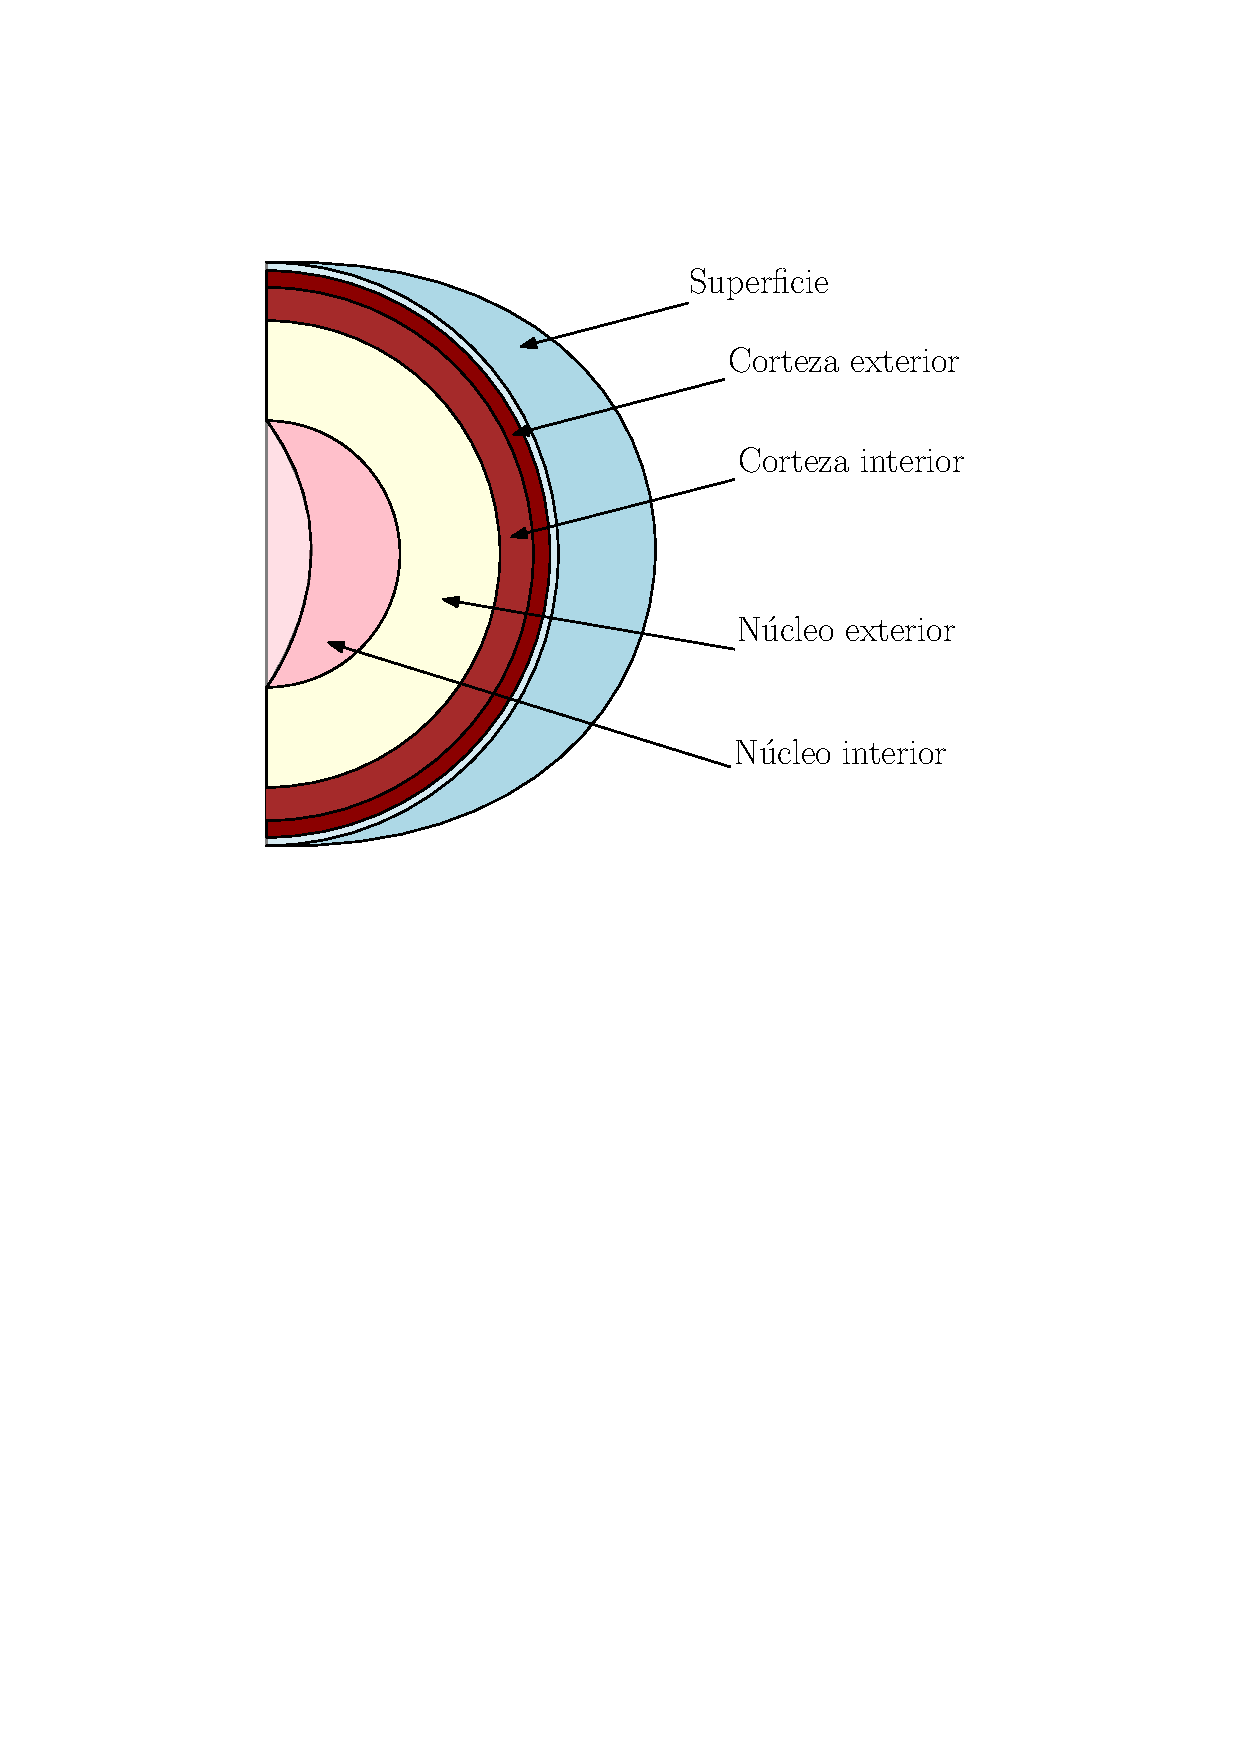
\includegraphics[width=200pt]{figures/neutronstar.pdf}
    \caption{Estructura interna de una estrella de neutrones}
    \label{NSS}
\end{figure}
\TODO{Llenar la imagen.}

\section{Criterios de estabilidad}

\subsection{Condición de estabilidad de Harrison-Zeldovich-Novikov}

\begin{equation}
    \frac { \partial M \left( \rho _ { c } \right) } { \partial \rho _ { c } } > 0
\end{equation}


\subsection{Condición de estabilidad por convección adiabática}

\begin{equation}
    \rho ^ { \prime \prime } ( r ) \leq 0
\end{equation}
